% Author: Xu Chen, University of Washington
% Lab 07 scene: drive D1 (demos): disk, actuator arm and VCM, the head over a track; the sampled track-following loop.
\documentclass[border=4pt]{standalone}
% Author: Xu Chen, University of Washington
% Shared TikZ style for the Control in Practice scene figures. % Author: Xu Chen, University of Washington
% Shared TikZ style for the Control in Practice scene figures. % Author: Xu Chen, University of Washington
% Shared TikZ style for the Control in Practice scene figures. \input{../../../docs/figures/cipstyle} from a lab.
\usepackage{amsmath,amssymb}
\usepackage[T1]{fontenc}
\usepackage{lmodern}
\usepackage{tikz}
\usepackage[siunitx]{circuitikz}
\usetikzlibrary{arrows.meta,calc,positioning,decorations.pathmorphing,decorations.markings,patterns,shapes.geometric,shadings,fit,backgrounds}
% restrained palette
\definecolor{ink}{HTML}{1A1A1A}
\definecolor{steel}{HTML}{8C96A0}
\definecolor{metal}{HTML}{D5DAE0}
\definecolor{accent}{HTML}{1F4E79}   % controller, signals we choose
\definecolor{plantc}{HTML}{FBE7D6}   % plant fill
\definecolor{sensorc}{HTML}{DCE8F3}  % sensor fill
\definecolor{dist}{HTML}{B03A2E}     % disturbances, forces from the environment
\definecolor{act}{HTML}{2E7D4F}      % actuation
\definecolor{note}{HTML}{555555}
\tikzset{
  every picture/.style={line width=0.8pt, >={Stealth[length=2.4mm]}, font=\small},
  thin line/.style={line width=0.5pt},
  thick line/.style={line width=1.2pt},
  dim/.style={thin line, note, {Stealth[length=1.6mm]}-{Stealth[length=1.6mm]}},
  ground/.style={pattern=north east lines, pattern color=steel, draw=none},
  block/.style={draw=ink, rounded corners=1.5pt, minimum height=9mm, minimum width=16mm, align=center, fill=white},
  plant/.style={block, fill=plantc},
  sensor/.style={block, fill=sensorc},
  ctrl/.style={block, draw=accent, text=accent, thick line},
  sum/.style={draw=ink, circle, minimum size=5mm, inner sep=0pt},
  sig/.style={->, ink},
  distsig/.style={->, dist, thick line},
  force/.style={-{Stealth[length=3mm]}, thick line},
  panel title/.style={font=\normalsize\bfseries, anchor=west, ink},
  caption/.style={font=\footnotesize, note, align=left},
}
 from a lab.
\usepackage{amsmath,amssymb}
\usepackage[T1]{fontenc}
\usepackage{lmodern}
\usepackage{tikz}
\usepackage[siunitx]{circuitikz}
\usetikzlibrary{arrows.meta,calc,positioning,decorations.pathmorphing,decorations.markings,patterns,shapes.geometric,shadings,fit,backgrounds}
% restrained palette
\definecolor{ink}{HTML}{1A1A1A}
\definecolor{steel}{HTML}{8C96A0}
\definecolor{metal}{HTML}{D5DAE0}
\definecolor{accent}{HTML}{1F4E79}   % controller, signals we choose
\definecolor{plantc}{HTML}{FBE7D6}   % plant fill
\definecolor{sensorc}{HTML}{DCE8F3}  % sensor fill
\definecolor{dist}{HTML}{B03A2E}     % disturbances, forces from the environment
\definecolor{act}{HTML}{2E7D4F}      % actuation
\definecolor{note}{HTML}{555555}
\tikzset{
  every picture/.style={line width=0.8pt, >={Stealth[length=2.4mm]}, font=\small},
  thin line/.style={line width=0.5pt},
  thick line/.style={line width=1.2pt},
  dim/.style={thin line, note, {Stealth[length=1.6mm]}-{Stealth[length=1.6mm]}},
  ground/.style={pattern=north east lines, pattern color=steel, draw=none},
  block/.style={draw=ink, rounded corners=1.5pt, minimum height=9mm, minimum width=16mm, align=center, fill=white},
  plant/.style={block, fill=plantc},
  sensor/.style={block, fill=sensorc},
  ctrl/.style={block, draw=accent, text=accent, thick line},
  sum/.style={draw=ink, circle, minimum size=5mm, inner sep=0pt},
  sig/.style={->, ink},
  distsig/.style={->, dist, thick line},
  force/.style={-{Stealth[length=3mm]}, thick line},
  panel title/.style={font=\normalsize\bfseries, anchor=west, ink},
  caption/.style={font=\footnotesize, note, align=left},
}
 from a lab.
\usepackage{amsmath,amssymb}
\usepackage[T1]{fontenc}
\usepackage{lmodern}
\usepackage{tikz}
\usepackage[siunitx]{circuitikz}
\usetikzlibrary{arrows.meta,calc,positioning,decorations.pathmorphing,decorations.markings,patterns,shapes.geometric,shadings,fit,backgrounds}
% restrained palette
\definecolor{ink}{HTML}{1A1A1A}
\definecolor{steel}{HTML}{8C96A0}
\definecolor{metal}{HTML}{D5DAE0}
\definecolor{accent}{HTML}{1F4E79}   % controller, signals we choose
\definecolor{plantc}{HTML}{FBE7D6}   % plant fill
\definecolor{sensorc}{HTML}{DCE8F3}  % sensor fill
\definecolor{dist}{HTML}{B03A2E}     % disturbances, forces from the environment
\definecolor{act}{HTML}{2E7D4F}      % actuation
\definecolor{note}{HTML}{555555}
\tikzset{
  every picture/.style={line width=0.8pt, >={Stealth[length=2.4mm]}, font=\small},
  thin line/.style={line width=0.5pt},
  thick line/.style={line width=1.2pt},
  dim/.style={thin line, note, {Stealth[length=1.6mm]}-{Stealth[length=1.6mm]}},
  ground/.style={pattern=north east lines, pattern color=steel, draw=none},
  block/.style={draw=ink, rounded corners=1.5pt, minimum height=9mm, minimum width=16mm, align=center, fill=white},
  plant/.style={block, fill=plantc},
  sensor/.style={block, fill=sensorc},
  ctrl/.style={block, draw=accent, text=accent, thick line},
  sum/.style={draw=ink, circle, minimum size=5mm, inner sep=0pt},
  sig/.style={->, ink},
  distsig/.style={->, dist, thick line},
  force/.style={-{Stealth[length=3mm]}, thick line},
  panel title/.style={font=\normalsize\bfseries, anchor=west, ink},
  caption/.style={font=\footnotesize, note, align=left},
}

\begin{document}
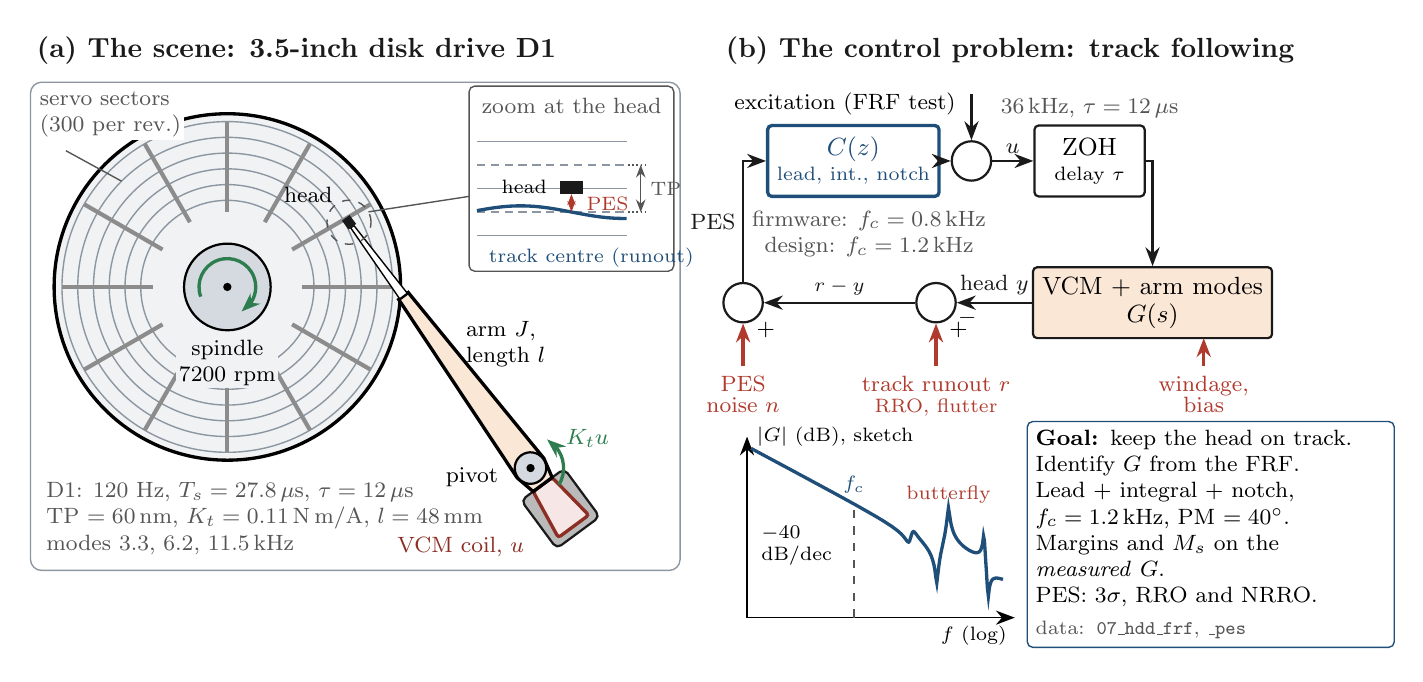
\begin{tikzpicture}
% ------------------------------------------------------------------ (a) the scene
\node[panel title] at (0,7.15) {(a) The scene: 3.5-inch disk drive D1};
% base plate
\draw[thin line, steel, rounded corners=4pt] (0.05,0.55) rectangle (8.3,6.75);
% disk platter with tracks and servo sectors
\coordinate (O) at (2.55,4.15);
\fill[metal!35] (O) circle (2.2);
\draw[thick line] (O) circle (2.2);
\foreach \r in {1.1,1.3,...,2.1} \draw[thin line, steel] (O) circle (\r);
\foreach \a in {0,30,...,330} \draw[line width=1.5pt, ink!50] ($(O)+(\a:0.95)$) -- ($(O)+(\a:2.1)$);
\fill[metal] (O) circle (0.55); \draw (O) circle (0.55); \fill (O) circle (1.5pt);
\draw[act, thick line, ->] ($(O)+(200:0.36)$) arc (200:-60:0.36);
\node[font=\footnotesize, anchor=north, align=center, fill=metal!35, inner sep=1pt] at ($(O)+(0,-0.62)$) {spindle\\7200 rpm};
\node[caption, anchor=north west, align=left, fill=white, inner sep=1pt] at (0.12,6.68) {servo sectors\\(300 per rev.)};
\draw[thin line, note] (0.5,5.88) -- ($(O)+(135:1.9)$);
% actuator in its own frame: pivot at the origin, x axis toward the head
\begin{scope}[shift={(6.400,1.850)}, rotate=126.441]
  \draw[fill=ink!30, draw=ink, rounded corners=2pt] (-1.02,-0.34) rectangle (-0.26,0.34);           % VCM magnet
  \draw[fill=dist!12, draw=dist!80!black, thick line, rounded corners=1pt] (-0.92,-0.24) -- (-0.26,-0.15)
        -- (-0.26,0.15) -- (-0.92,0.24) -- cycle;                                                  % coil
  \draw[fill=plantc, thick line] (-0.26,-0.15) -- (0,-0.21) -- (2.716,-0.075) -- (2.716,0.075) -- (0,0.21) -- (-0.26,0.15) -- cycle;  % arm
  \draw[fill=white, thin line] (2.716,-0.06) -- (3.810,-0.025) -- (3.810,0.025) -- (2.716,0.06) -- cycle;   % suspension
  \fill[ink] (3.810,-0.06) rectangle (3.950,0.06);                                                   % slider with the head
  \fill[metal] (0,0) circle (0.2); \draw (0,0) circle (0.2); \fill (0,0) circle (1.5pt);
\end{scope}
\coordinate (P) at (6.400,1.850);
\coordinate (H) at (4.095,4.972);
\draw[act, thick line, ->] ($(P)+(-30:0.42)$) arc (-30:60:0.42);
\node[act, font=\footnotesize, anchor=west] at ($(P)+(0.32,0.38)$) {$K_t u$};
\node[font=\footnotesize, anchor=east] at ($(P)+(-0.28,-0.12)$) {pivot};
\node[font=\footnotesize, anchor=east, dist!80!black] at (6.45,0.85) {VCM coil, $u$};
\node[font=\footnotesize, anchor=south west, align=left] at (5.45,3.0) {arm $J$,\\length $l$};
\node[font=\footnotesize, anchor=south east] at ($(H)+(-0.08,0.12)$) {head};
\draw[thin line, note, dashed] (H) circle (0.28);
\draw[thin line, note] ($(H)+(28:0.28)$) -- (5.62,5.3);
% zoom inset: tracks, head offset, PES
\begin{scope}[shift={(5.62,4.35)}]
  \draw[thin line, note, rounded corners=2pt, fill=white] (0,0) rectangle (2.6,2.35);
  \node[caption, anchor=north west] at (0.03,2.33) {zoom at the head};
  \foreach \y in {0.45,1.05,1.65} \draw[thin line, steel] (0.1,\y) -- (2.0,\y);
  \foreach \y in {0.75,1.35} \draw[thin line, steel, densely dashed] (0.1,\y) -- (2.0,\y);
  \foreach \y in {0.75,1.35} \draw[thin line, note, densely dotted] (2.02,\y) -- (2.26,\y);
  \draw[accent, thick line] plot[domain=0.1:2.0, samples=50] (\x, {0.75+0.08*sin(deg(2.4*\x))});
  \fill[ink] (1.15,0.98) rectangle (1.45,1.14);
  \node[font=\scriptsize, anchor=east] at (1.12,1.07) {head};
  \draw[dist, thick line, {Stealth[length=1.4mm]}-{Stealth[length=1.4mm]}] (1.3,{0.75+0.08*sin(deg(2.4*1.3))}) -- (1.3,0.98);
  \node[font=\scriptsize, dist, anchor=west] at (1.36,0.86) {PES};
  \draw[dim] (2.18,0.75) -- (2.18,1.35) node[midway, right=0pt, font=\scriptsize] {TP};
  \node[font=\scriptsize, accent, anchor=north west] at (0.12,0.42) {track centre (runout)};
\end{scope}
\node[caption, anchor=south west, align=left] at (0.12,0.62) {D1: 120 Hz, $T_s = 27.8\,\mu$s, $\tau = 12\,\mu$s\\TP $=60$\,nm, $K_t=0.11$\,N\,m/A, $l=48$\,mm\\modes 3.3, 6.2, 11.5\,kHz};

% ------------------------------------------------------------------ (b) the control problem
\begin{scope}[shift={(8.75,0)}]
\node[panel title] at (0,7.15) {(b) The control problem: track following};
\def\ya{5.75} \def\yb{3.95}
\node[ctrl, minimum width=17mm, align=center] (C) at (1.75,\ya) {$C(z)$\\[-2pt]{\scriptsize lead, int., notch}};
\node[sum] (s2) at (3.25,\ya) {};
\node[block, minimum width=14mm, align=center] (zoh) at (4.75,\ya) {ZOH\\[-2pt]{\scriptsize delay $\tau$}};
\node[plant, minimum width=24mm, align=center] (G) at (5.55,\yb) {VCM + arm modes\\[-1pt]$G(s)$};
\node[sum] (s3) at (2.8,\yb) {};
\node[sum] (s4) at (0.35,\yb) {};
\draw[sig] (C) -- (s2);
\draw[sig] (s2) -- node[above=-1pt, font=\footnotesize] {$u$} (zoh);
\draw[sig] (zoh) -| (G);
\draw[sig] (G) -- node[above=-1pt, font=\footnotesize] {head $y$} node[pos=0.86, below=-1pt, font=\footnotesize] {$-$} (s3);
\draw[sig] (s3) -- node[above=-1pt, font=\scriptsize] {$r - y$} (s4);
\draw[sig] (s4) |- node[pos=0.25, left=-1pt, font=\footnotesize] {PES} (C);
\node[font=\footnotesize, anchor=north west] at (2.84,\yb-0.12) {$+$};
\draw[distsig] (2.8,\yb-0.8) node[below, font=\footnotesize, dist, align=center] {track runout $r$\\[-2pt]{\scriptsize RRO, flutter}} -- (s3);
\node[font=\footnotesize, anchor=north west] at (0.39,\yb-0.12) {$+$};
\draw[distsig] (0.35,\yb-0.8) node[below, font=\footnotesize, dist, align=center] {PES\\[-2pt]noise $n$} -- (s4);
\draw[distsig] (6.2,\yb-0.8) node[below, font=\footnotesize, dist, align=center] {windage,\\[-2pt]bias} -- (6.2,\yb-0.45);
\draw[sig] (3.25,\ya+0.85) -- (s2);
\node[font=\footnotesize, anchor=east] at (3.18,\ya+0.72) {excitation (FRF test)};
\node[caption, anchor=south, align=center] at (4.75,\ya+0.42) {36\,kHz, $\tau=12\,\mu$s};
\node[caption, anchor=north, align=center] at (1.95,\ya-0.5) {firmware: $f_c=0.8$\,kHz\\design: $f_c=1.2$\,kHz};
% Bode magnitude sketch: rigid body and the resonances
\begin{scope}[shift={(0,-0.35)}]
  \draw[->, thin line] (0.4,0.3) -- (3.8,0.3) node[below left=-1pt, font=\scriptsize] {$f$ (log)};
  \draw[->, thin line] (0.4,0.3) -- (0.4,2.6) node[right, font=\scriptsize] {$|G|$ (dB), sketch};
  \draw[accent, thick line] plot coordinates {(0.450,2.450) (0.462,2.443) (0.475,2.437) (0.487,2.430) (0.499,2.424) (0.512,2.417) (0.524,2.410) (0.536,2.404) (0.549,2.397) (0.561,2.390) (0.574,2.384) (0.586,2.377) (0.598,2.371) (0.611,2.364) (0.623,2.357) (0.635,2.351) (0.648,2.344) (0.660,2.337) (0.672,2.331) (0.685,2.324) (0.697,2.318) (0.709,2.311) (0.722,2.304) (0.734,2.298) (0.747,2.291) (0.759,2.284) (0.771,2.278) (0.784,2.271) (0.796,2.265) (0.808,2.258) (0.821,2.251) (0.833,2.245) (0.845,2.238) (0.858,2.231) (0.870,2.225) (0.882,2.218) (0.895,2.212) (0.907,2.205) (0.919,2.198) (0.932,2.192) (0.944,2.185) (0.957,2.178) (0.969,2.172) (0.981,2.165) (0.994,2.158) (1.006,2.152) (1.018,2.145) (1.031,2.139) (1.043,2.132) (1.055,2.125) (1.068,2.119) (1.080,2.112) (1.092,2.105) (1.105,2.099) (1.117,2.092) (1.130,2.085) (1.142,2.079) (1.154,2.072) (1.167,2.065) (1.179,2.059) (1.191,2.052) (1.204,2.045) (1.216,2.039) (1.228,2.032) (1.241,2.025) (1.253,2.019) (1.265,2.012) (1.278,2.005) (1.290,1.999) (1.303,1.992) (1.315,1.985) (1.327,1.979) (1.340,1.972) (1.352,1.965) (1.364,1.959) (1.377,1.952) (1.389,1.945) (1.401,1.939) (1.414,1.932) (1.426,1.925) (1.438,1.919) (1.451,1.912) (1.463,1.905) (1.475,1.898) (1.488,1.892) (1.500,1.885) (1.513,1.878) (1.525,1.872) (1.537,1.865) (1.550,1.858) (1.562,1.851) (1.574,1.845) (1.587,1.838) (1.599,1.831) (1.611,1.824) (1.624,1.818) (1.636,1.811) (1.648,1.804) (1.661,1.797) (1.673,1.790) (1.686,1.784) (1.698,1.777) (1.710,1.770) (1.723,1.763) (1.735,1.756) (1.747,1.749) (1.760,1.743) (1.772,1.736) (1.784,1.729) (1.797,1.722) (1.809,1.715) (1.821,1.708) (1.834,1.701) (1.846,1.694) (1.858,1.687) (1.871,1.680) (1.883,1.673) (1.896,1.666) (1.908,1.659) (1.920,1.652) (1.933,1.645) (1.945,1.638) (1.957,1.631) (1.970,1.624) (1.982,1.617) (1.994,1.610) (2.007,1.603) (2.019,1.595) (2.031,1.588) (2.044,1.581) (2.056,1.574) (2.069,1.566) (2.081,1.559) (2.093,1.551) (2.106,1.544) (2.118,1.536) (2.130,1.529) (2.143,1.521) (2.155,1.513) (2.167,1.505) (2.180,1.497) (2.192,1.489) (2.204,1.481) (2.217,1.473) (2.229,1.465) (2.242,1.456) (2.254,1.447) (2.266,1.438) (2.279,1.429) (2.291,1.420) (2.303,1.410) (2.316,1.400) (2.328,1.390) (2.340,1.379) (2.353,1.367) (2.365,1.355) (2.377,1.342) (2.390,1.328) (2.402,1.312) (2.414,1.296) (2.427,1.279) (2.439,1.265) (2.452,1.259) (2.464,1.273) (2.476,1.310) (2.489,1.354) (2.501,1.385) (2.513,1.393) (2.526,1.387) (2.538,1.373) (2.550,1.357) (2.563,1.340) (2.575,1.324) (2.587,1.308) (2.600,1.293) (2.612,1.278) (2.625,1.263) (2.637,1.247) (2.649,1.232) (2.662,1.216) (2.674,1.199) (2.686,1.181) (2.699,1.162) (2.711,1.141) (2.723,1.117) (2.736,1.091) (2.748,1.059) (2.760,1.022) (2.773,0.974) (2.785,0.909) (2.797,0.816) (2.810,0.743) (2.822,0.842) (2.835,0.952) (2.847,1.036) (2.859,1.105) (2.872,1.166) (2.884,1.224) (2.896,1.282) (2.909,1.343) (2.921,1.413) (2.933,1.498) (2.946,1.607) (2.958,1.694) (2.970,1.620) (2.983,1.532) (2.995,1.471) (3.008,1.425) (3.020,1.389) (3.032,1.360) (3.045,1.335) (3.057,1.313) (3.069,1.295) (3.082,1.278) (3.094,1.262) (3.106,1.248) (3.119,1.235) (3.131,1.223) (3.143,1.212) (3.156,1.201) (3.168,1.192) (3.181,1.182) (3.193,1.174) (3.205,1.166) (3.218,1.158) (3.230,1.151) (3.242,1.145) (3.255,1.139) (3.267,1.134) (3.279,1.130) (3.292,1.127) (3.304,1.125) (3.316,1.125) (3.329,1.127) (3.341,1.132) (3.353,1.141) (3.366,1.157) (3.378,1.186) (3.391,1.238) (3.403,1.337) (3.415,1.277) (3.428,1.067) (3.440,0.885) (3.452,0.682) (3.465,0.571) (3.477,0.673) (3.489,0.731) (3.502,0.762) (3.514,0.781) (3.526,0.792) (3.539,0.798) (3.551,0.802) (3.564,0.803) (3.576,0.803) (3.588,0.801) (3.601,0.799) (3.613,0.796) (3.625,0.793) (3.638,0.789) (3.650,0.785)};
  \draw[thin line, note, dashed] (1.758,0.3) -- (1.758,1.75) node[above, font=\scriptsize, accent] {$f_c$};
  \node[font=\scriptsize, anchor=north west, align=left] at (0.45,1.6) {$-40$\\dB/dec};
  \node[font=\scriptsize, dist, anchor=south] at (2.96,1.62) {butterfly};
\end{scope}
% goal / data box
\node[draw=accent, thin line, rounded corners=2pt, fill=white, align=left, anchor=north west, font=\footnotesize,
      text width=4.45cm, inner sep=3pt] at (3.95,2.45)
  {\textbf{Goal:} keep the head on track.\\Identify $G$ from the FRF.\\Lead + integral + notch,\\$f_c=1.2$\,kHz, PM $=40^\circ$.\\Margins and $M_s$ on the\\\emph{measured} $G$.\\PES: $3\sigma$, RRO and NRRO.\\[2pt]{\scriptsize\color{note}data: \texttt{07\_hdd\_frf}, \texttt{\_pes}}};
\end{scope}
\end{tikzpicture}
\end{document}
